\documentclass{beamer}
\usepackage{transparent}
\usepackage[beamer]{shortcut}


\usepackage[autoplay]{animate}
\usepackage{bibentry}
\usepackage{subcaption}
\usepackage{stackengine}
\usepackage{appendixnumberbeamer}

\graphicspath{{./images/}}
\def\TikzLocation{./tikz/}
\def\tkzscl{1}

\def\stackalignment{l}


\definecolor{primary}{RGB}{191,213,219}
\definecolor{secondary}{RGB}{144,106,66}
\setbeamercolor{block title}{fg=darkred}
\newcommand{\btitle}[1]{{\usebeamerfont{block title}\usebeamercolor[fg]{block title} #1}}

\AtBeginSection[]
{
}


\makeatletter
\def\beamer@newblock{%
  \usebeamercolor[fg]{bibliography entry author}%
  \usebeamerfont{bibliography entry author}%
  \usebeamertemplate{bibliography entry author}%
  \def\newblock{%
    \usebeamercolor[fg]{bibliography entry title}%
    \usebeamerfont{bibliography entry title}%
    \usebeamertemplate{bibliography entry title}%
    \def\newblock{%
      \usebeamercolor[fg]{bibliography entry location}%
      \usebeamerfont{bibliography entry location}%
      \usebeamertemplate{bibliography entry location}%
      \def\newblock{%
        \usebeamercolor[fg]{bibliography entry note}%
        \usebeamerfont{bibliography entry note}%
        \usebeamertemplate{bibliography entry note}}}}%
  \leavevmode\setbox\beamer@tempbox=\hbox{}\ht\beamer@tempbox=0em\box\beamer@tempbox}
  \setbeamertemplate{bibliography entry title}{}{}

\makeatother

\usepackage[square, authoryear]{natbib}


%-----------------------------------------------------------------------------
%	CUSTOM COMANDS
%-----------------------------------------------------------------------------

\def\keypoint#1{\hspace{0pt plus 1 filll}\textcolor{gray}{[{\color{linkcolor}#1}]}~}
\def\mycite#1{\keypoint{\small\citealt{#1}}}
\def\citeconf#1#2{
    {\textcolor{gray}[}%
        {\color{linkcolor}\citealt{#1}, #2}%
    {\textcolor{gray}]}}
\def\citeconfright#1#2{\hspace{0pt plus 1 filll}{\small\citeconf{#1}{#2}~}}
\def\biblio{
	\nobibliography{../../library}
	\def\biblio{}
}

\def\myitem{\hskip1ex{\color{linkcolor} $\blacktriangleright$}\hskip.3em}


\def\extraLogo{\includegraphics[width=.2\linewidth]{brain_and_signals}}


\newlength\bodywd
\newlength\skipg
\setlength\skipg{\widthof{\bf g}}
\newcommand{\techterm}[1]{
    \column{\widthof{\bf #1}}
    \centering
    \begin{beamercolorbox}[rounded=true, shadow=true]{title}
        \bf \phantom{g}\hskip-\skipg #1
    \end{beamercolorbox}
}

\pgfkeys{
    /highlight/.cd,
    c/.initial={darkred},
    wd/.initial={0}
}

\newcommand{\highlight}[2][]{%
    \pgfkeys{/highlight/.cd,#1}%
    \ifthenelse{\pgfkeysvalueof{/highlight/wd}=0}{
        \setlength\bodywd{\widthof{\bf #2}}
    }{
        \setlength\bodywd{\pgfkeysvalueof{/highlight/wd}}
    }
    \raisebox{-.5em}{
        \begin{beamercolorbox}[rounded=true, shadow=true, wd=\bodywd]{title}
            \centering\bf\phantom{g}\hskip-\skipg \textcolor{\pgfkeysvalueof{/highlight/c}}{#2}
    \end{beamercolorbox}}
}

\newcommand{\overimg}[5][.8\linewidth]{
    \begin{tikzpicture}
    \only<#2-#4>{%
        \node[inner sep=0em, outer sep=0em] (img) {\includegraphics[width=#1]{#3}};
    }%
    \only<#4>{%
        \path let
          \p1=($(img.north) - (0, 1em)$), \p2=(img.south)
          in
          node {\includegraphics[height=\y1-\y2]{#5}};
    }%
    \end{tikzpicture}
}


\institute{Concours CRCN Inria Saclay}
\author{Thomas Moreau}
\title{Apprentissage non-supervisé pour les signaux multivariés
       en neurosciences}


\setbeamertemplate{title page}[frame]


\begin{document}

\begin{frame}[plain]

\vskip.1\textheight
\begin{beamercolorbox}[sep=2pt,center, wd=\textwidth]{separationline}
    %Title box
    \begin{beamercolorbox}[center, wd=\SizeTitleBox]{headline}
        \begin{center}
            \centering
            \usebeamercolor{title}{\color{fg}\Large\textbf{{\inserttitle}}\hskip2em\\[1.5ex]}
            \usebeamercolor{author}{\color{fg}\small{\insertauthor}} -- %
            \usebeamercolor{institute}{\color{fg}\small{\insertinstitute}\\} 
        \end{center}
    \end{beamercolorbox}
    \vskip-1em
    \hskip0em
    % Separation line
    \begin{beamercolorbox}[center, wd=\SizeTitleBox]{separation line}\rule{0pt}{2pt}\end{beamercolorbox}\vfill
\end{beamercolorbox}
% LOGO and join work part of the title frame
\vskip2em
\begin{columns}[c]
    \column{.5\textwidth}
    \centering
        \includegraphics[width=.7\linewidth]{brain_and_signals}
    \column{.5\textwidth}
        \includeLogo{logo_inria}\\[1em]
        \includeLogo{logo_parietal}
\end{columns}


\biblio{}
\end{frame}

\def\biblio{}

%===========================================================================
\section{Me}
%===========================================================================

\begin{frame}[t]{Parcours}

\begin{columns}[c]
    \column{1em}
    \rotatebox{90}{\Large Formation}
    \column{.9\textwidth}
\begin{list}{}{\leftmargin=0em \itemsep=0em}
    \item 2010-2014: Ecole Polytechnique - Math App/Info
    \item 2013-2014: Double diplome Telecom ParisTech - Master MVA
\end{list}
    \begin{beamercolorbox}[rounded=true, shadow=true]{title}
       Apprentissage statistique, Traitement du signal et des images.
    \end{beamercolorbox}
\end{columns}

\vskip1em

\begin{columns}[c]
    \column{1em}
    \rotatebox{90}{\Large Recherche}
    \column{.9\textwidth}
    \begin{list}{}{\leftmargin=0em \itemsep=1em}
        \item 2014-2017: Thèse -- ENS Cachan (N. Vayatis \& L. Oudre)
        \vskip-.5em
        \begin{columns}[T]
            \column{.45\textwidth}
        \begin{block}{Maths appliquées}\footnotesize
            Optimisation distribuée\\
            Apprentissage non-supervisé\\
            Apprentissage de représentation
        \end{block}
        \column{.01\textwidth}
        \column{.45\textwidth}
        \begin{block}{Santé}\footnotesize
            Analyse de la marche\\
            Enregistrements oculomoteurs
        \end{block}
    
        \end{columns}
        
        \item 2018-2019: Post-doctorat -- Inria (équipe Parietal)
        \begin{beamercolorbox}[rounded=true, shadow=true]{title}
            Apprentissage de dictionnaire convolutif pour la MEG.\\
            \hskip3ex\color{black}$\Rightarrow$ Analyse de la structure locale des signaux
        \end{beamercolorbox}
    \end{list}
\end{columns}

\end{frame}


\begin{frame}{Analyse de l'équilibre dynamique}

\begin{columns}[T]
    \column{.6\textwidth}
    \centering
        \begin{columns}[c]
            \column{.4\linewidth}
            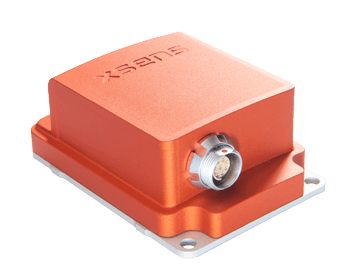
\includegraphics[width=\linewidth]{xsens}
            \column{.6\linewidth}
            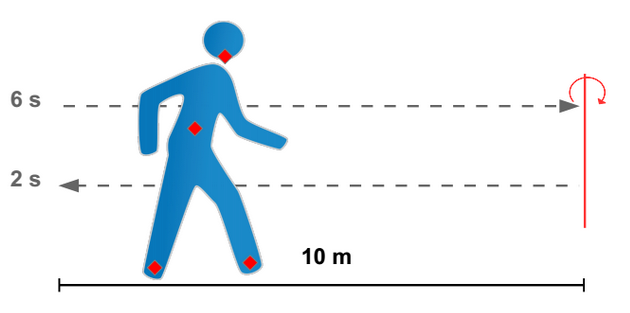
\includegraphics[width=\linewidth]{exo_marche}
        \end{columns}
        \vskip1em
        \alt<-2>{
            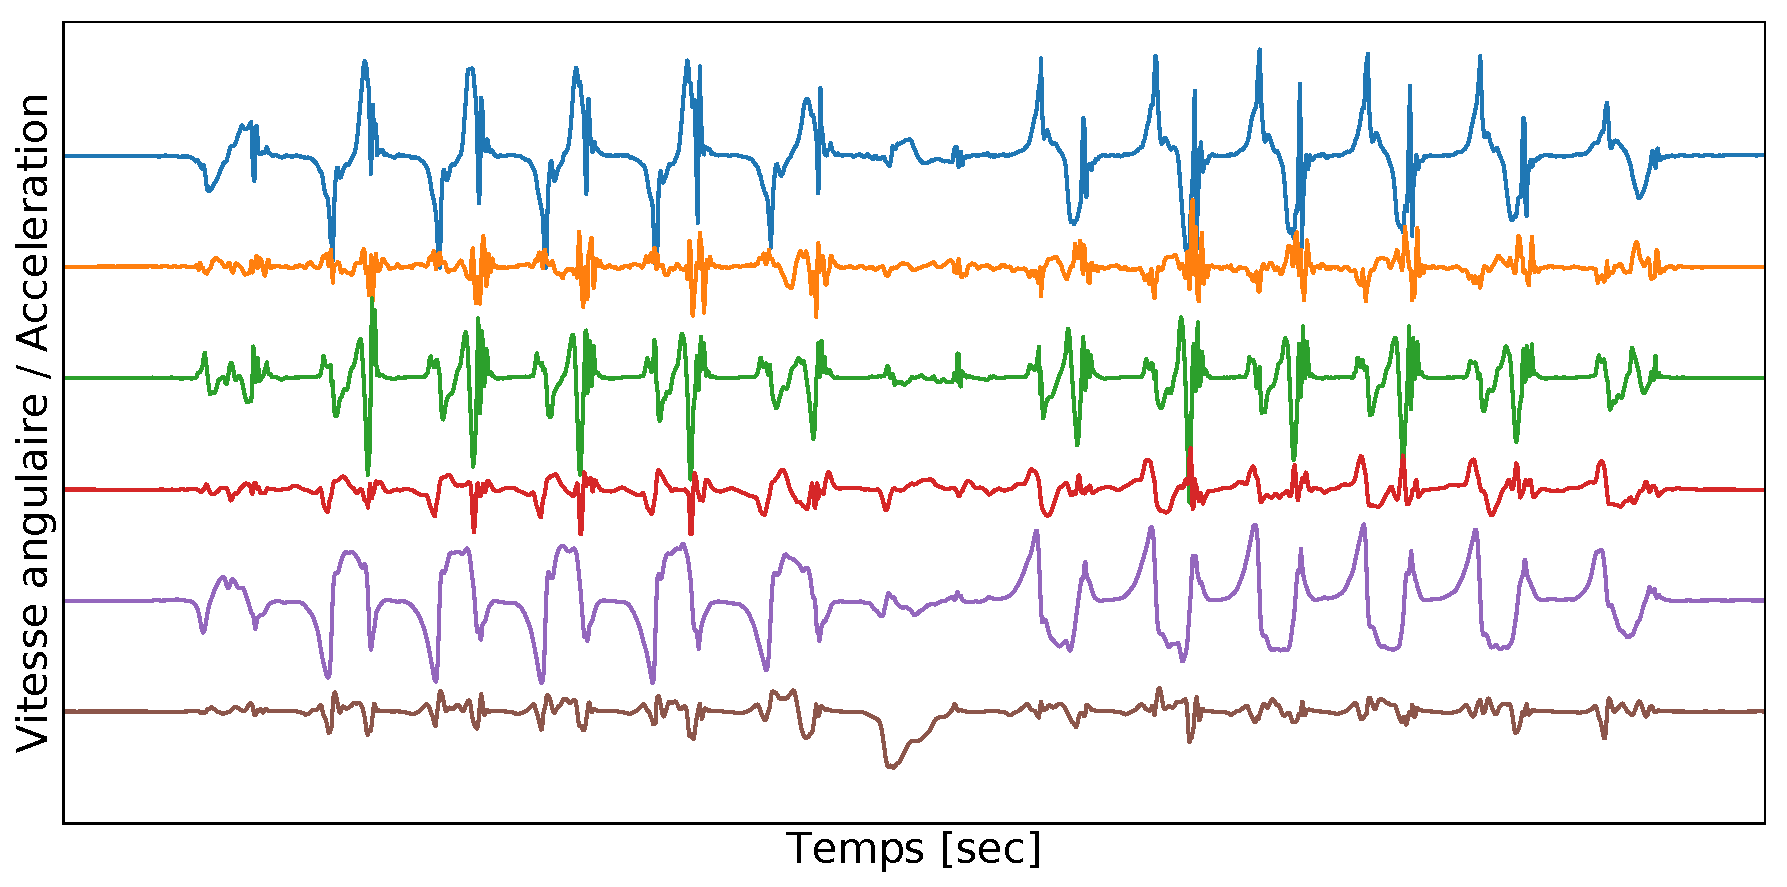
\includegraphics[width=\linewidth]{accelero}
        }{
            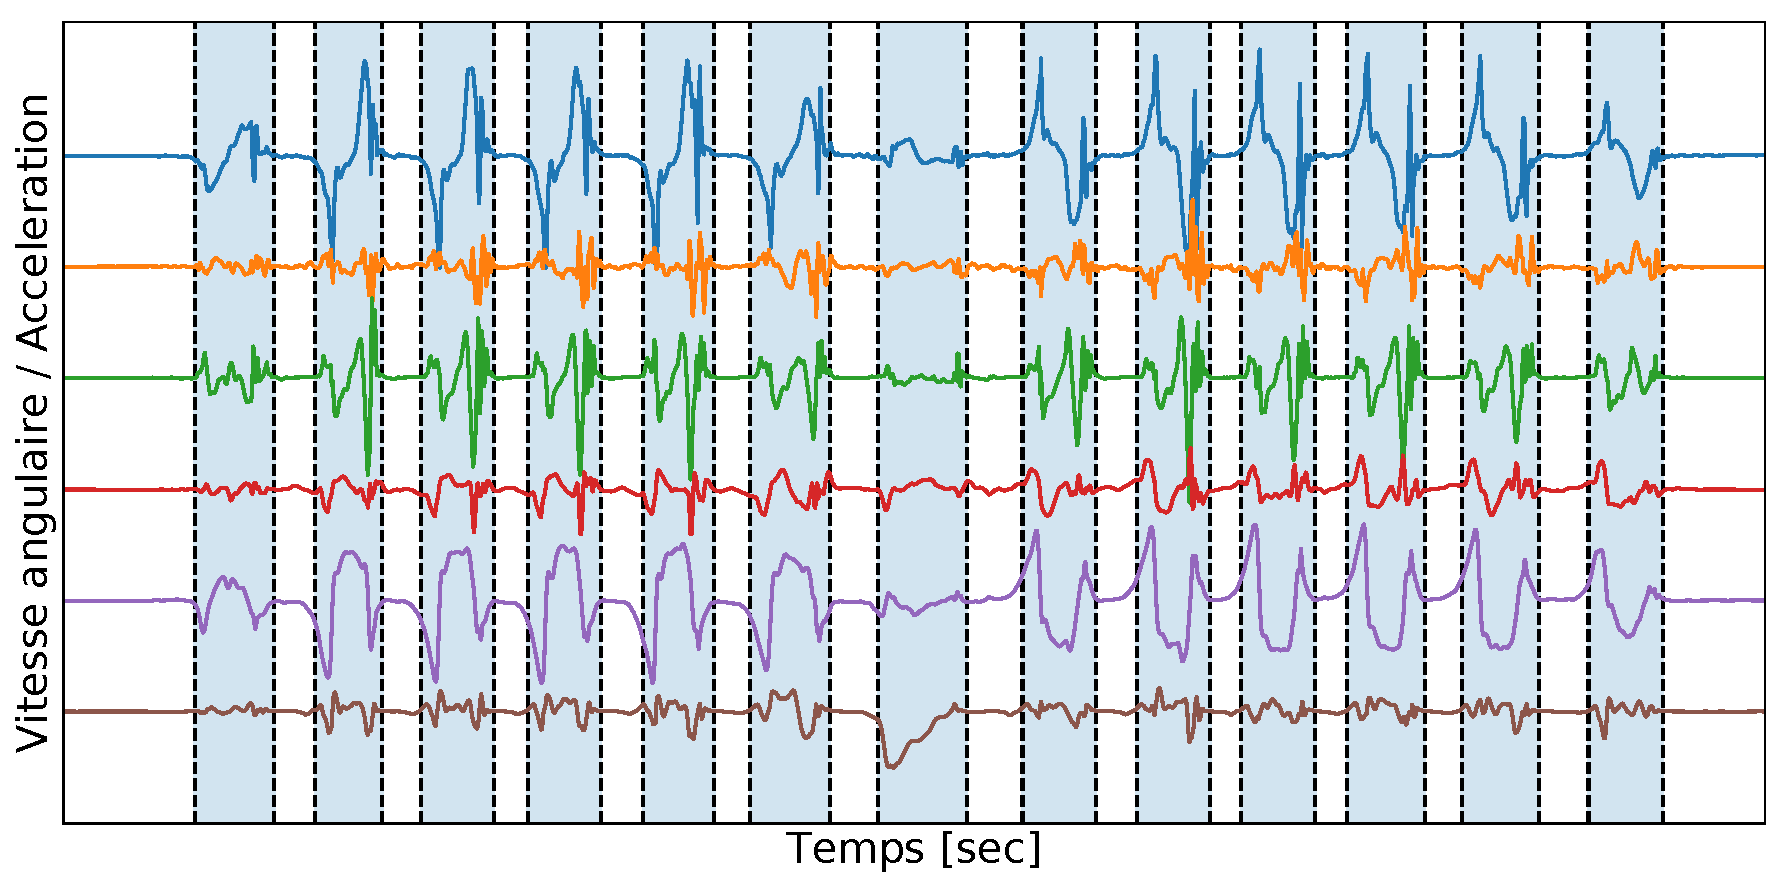
\includegraphics[width=\linewidth]{accelero_steps}
        }
        \uncover<4>{
            \vskip-1em\hskip.5ex
            \begin{beamercolorbox}[rounded=true, shadow=true, wd=.95\linewidth]{title}
                \textbf{Brevet:~} Segmentation de pas\\
                \textbf{Articles:} %
                    \textcolor{linkcolor}{Sensors 2018; PLoS One 2016}\\
            \end{beamercolorbox}
        }
    \column{.4\textwidth}
        \alt<1>{
            \vskip3em
            \begin{block}{Objectifs}
                \vskip.5em{\bf Quantifier l'équilibre}
                \begin{itemize}\itemsep.5em
                    \item Prédiction de chutes
                    \item Suivi de neuropathie
                    \item Suivi de rééducation
                \end{itemize}
               \vskip-.7em\textcolor{white}{.}
            \end{block}
        }{
            \begin{block}{Challenges}
                \vskip.5em
                Annotations faibles\\[.5em]
                Pas de comparaison canonique
                \vskip-.7em\textcolor{white}{.}
            \end{block}
            \begin{block}{Comparaison des signaux}
                \vskip.5em
                Représentation adaptée\\[.5em]
                $\Rightarrow$~Segmentation des pas.\\[.5em]
                Utiliser la {\bf structure locale} du signal.
                \vskip-.7em\textcolor{white}{.}
            \end{block}
        }
    \end{columns}

\end{frame}


\begin{frame}{Domaines d'application}{}


    \only<1-2>{
        {\large \bf Enregistrement inertiel}\\[1em]
        \centering
        \overimg{1}{accelero}{2}{accelero_dict}\\[1em]
        \textcolor{gray}{[\textcolor{linkcolor}{PLoS ONE 2016; Sensors 2018}]}
    }
    \only<3-4>{
        {\large \bf Image du Télescope Hubble}\\[1em]
        \centering
        \overimg{3}{Hubble}{4}{Hubble_dict}\\[1em]
        \textcolor{gray}{[\textcolor{linkcolor}{preprint 2019}]}
    }
    \only<5->{
        {\large \bf Magnétoencéphalographie (MEG)}\\[1em]
        \begin{columns}
            \column{.4\textwidth}
                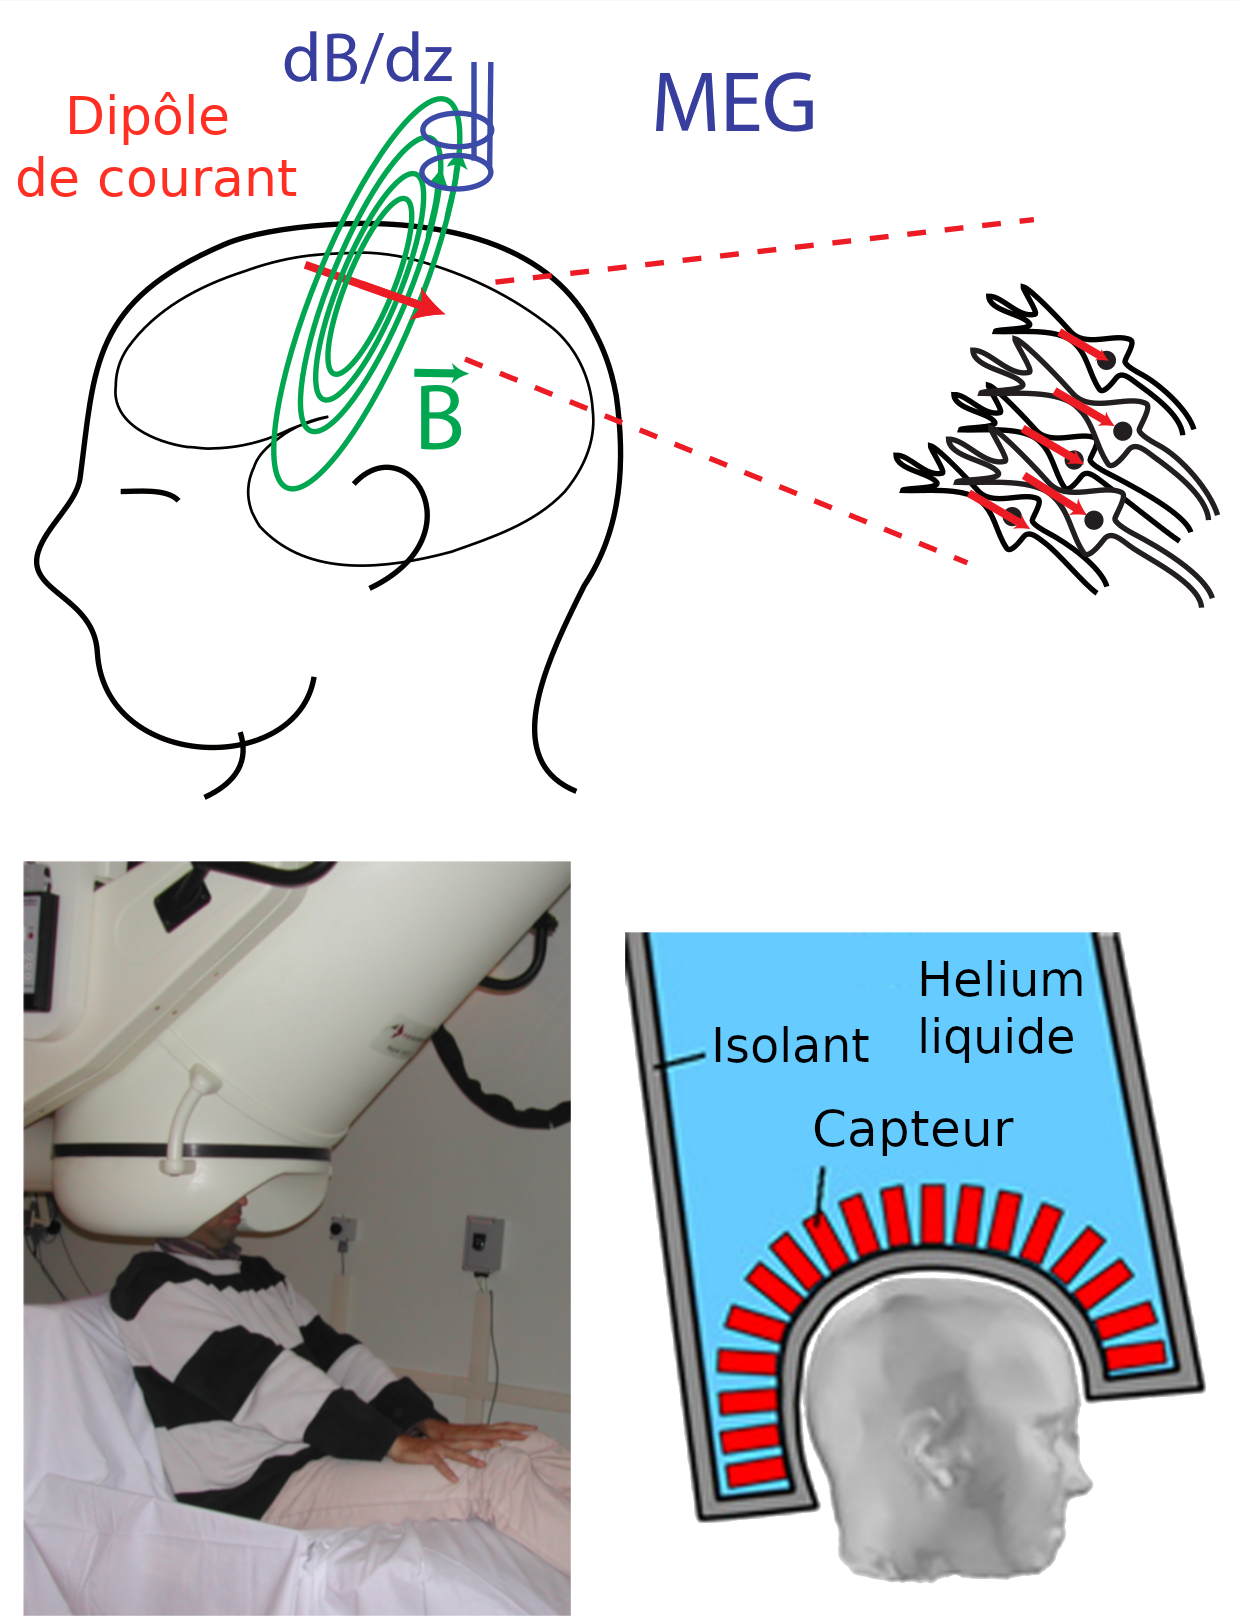
\includegraphics[height=.7\textheight]{meg_presentation}\\
            \column{.6\textwidth}
                \centering\highlight[c=linkcolor]{Structure locale invisible}\\
                \overimg[\linewidth]{5}{meg_signal}{6}{meg_dict}
        \end{columns}

    }
\end{frame}

\begin{frame}[t]{Structure locale des signaux}
    \vskip1.5em%
    \centering%
    \only<1>{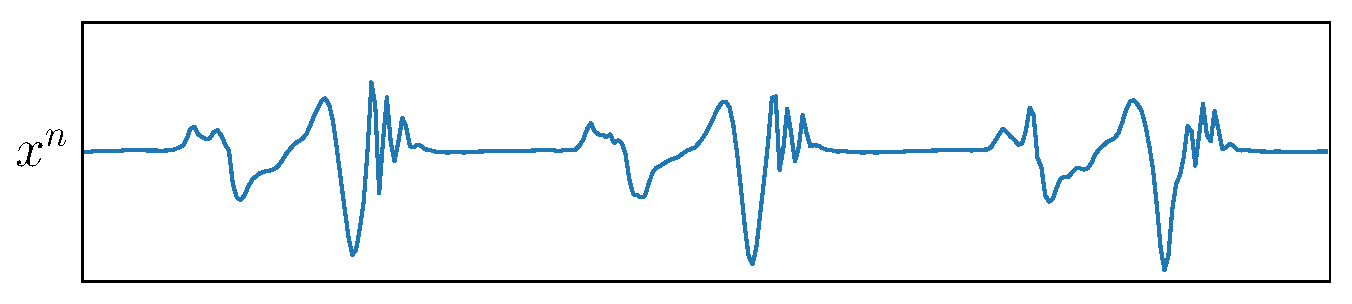
\includegraphics[width=\textwidth]{intro_csc_0}}%
    \only<2>{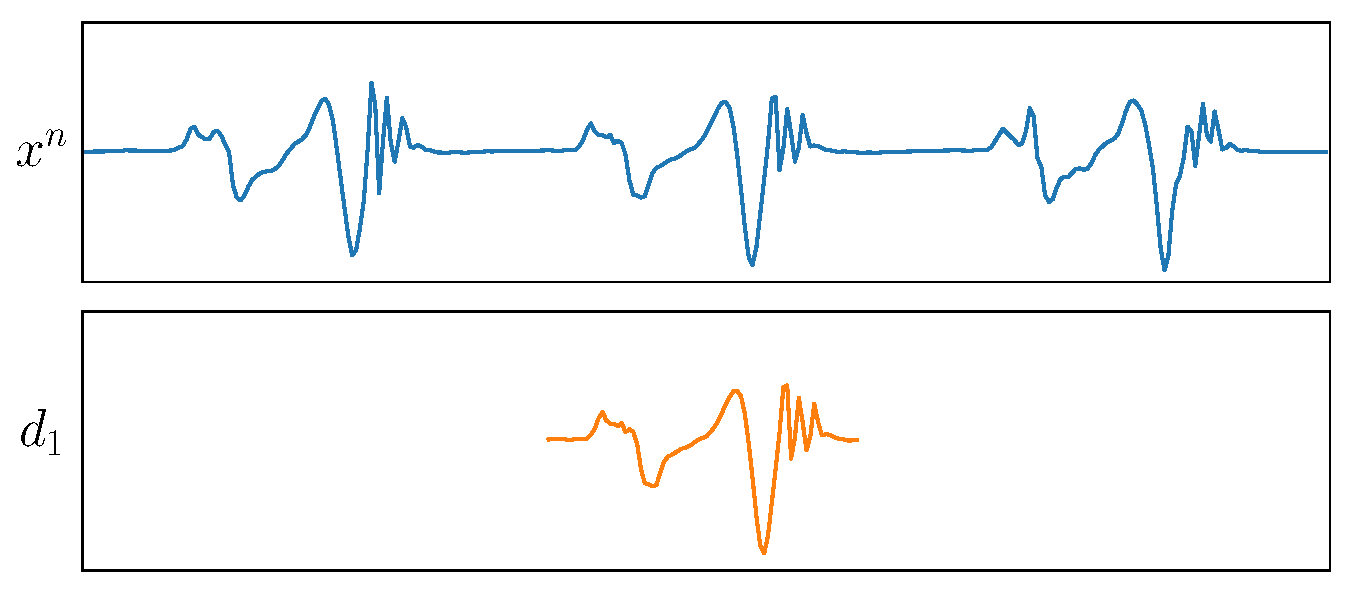
\includegraphics[width=\textwidth]{intro_csc_1}}%
    \only<3>{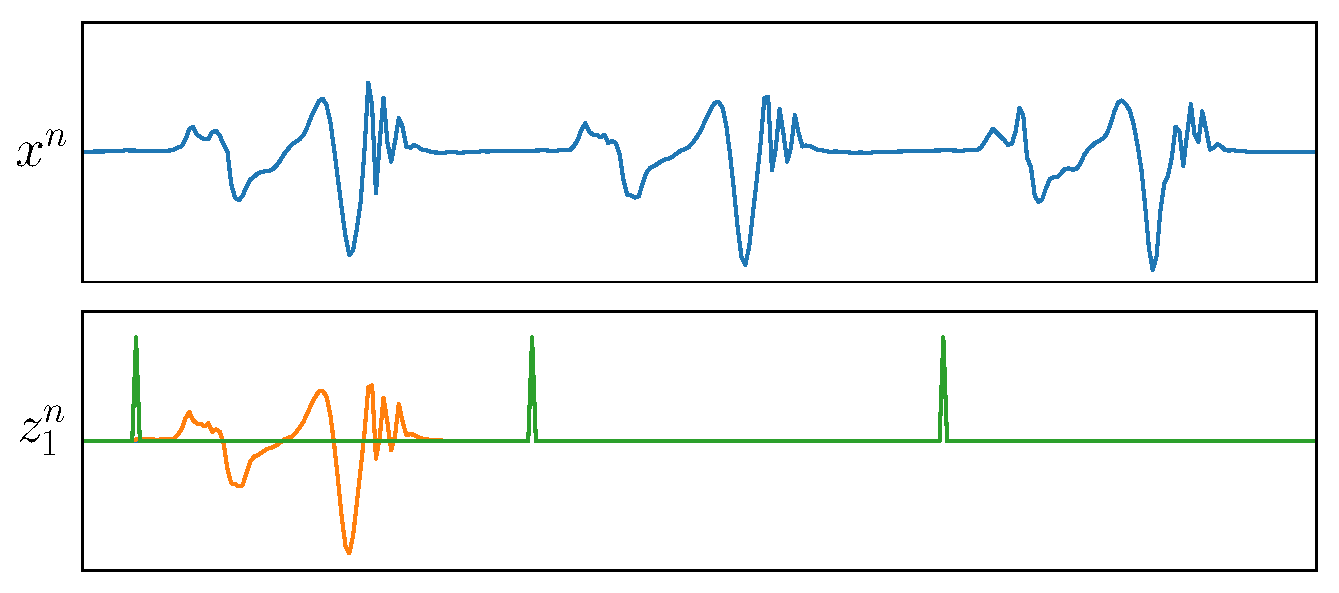
\includegraphics[width=\textwidth]{intro_csc_2}}%
    \only<4>{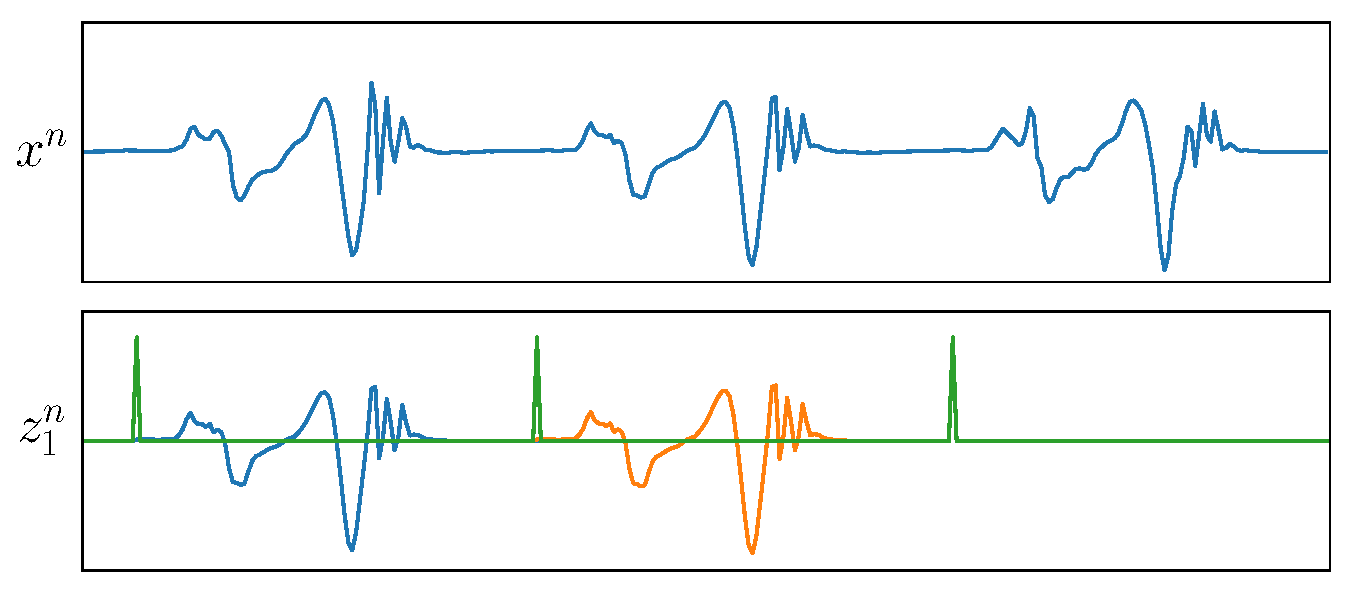
\includegraphics[width=\textwidth]{intro_csc_3}}%
    \only<5>{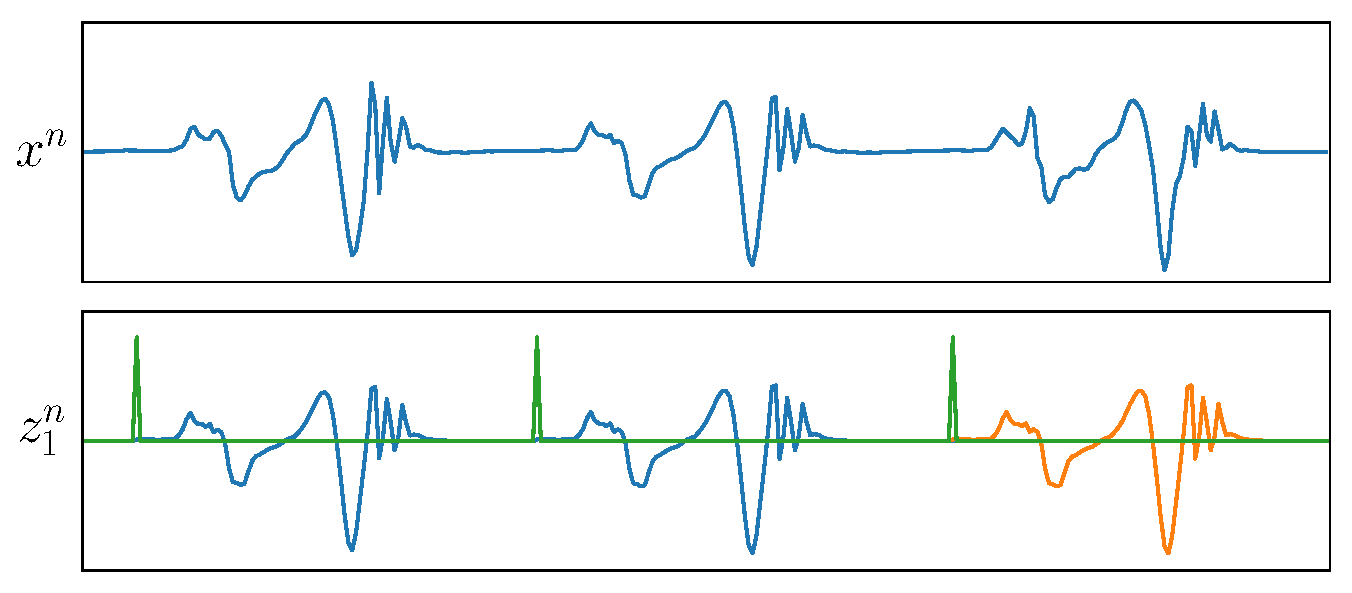
\includegraphics[width=\textwidth]{intro_csc_4}}%
    \only<6->{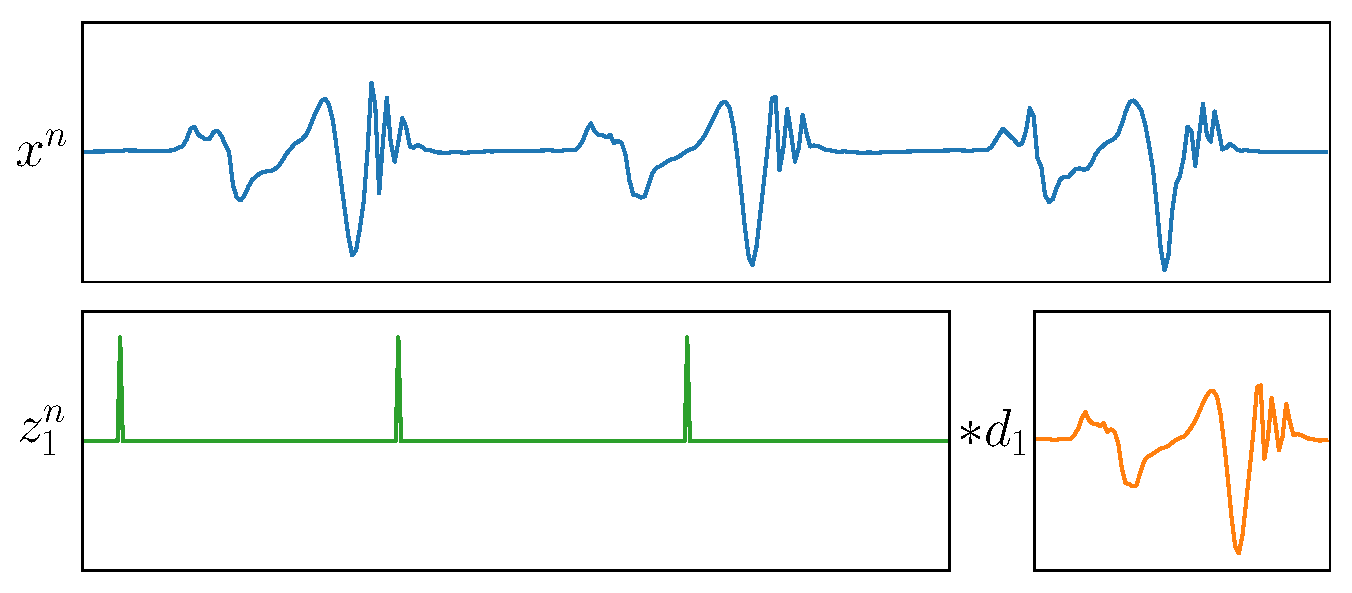
\includegraphics[width=\textwidth]{intro_csc_5}}%
    \vskip.2em%
    \only<7>{%
        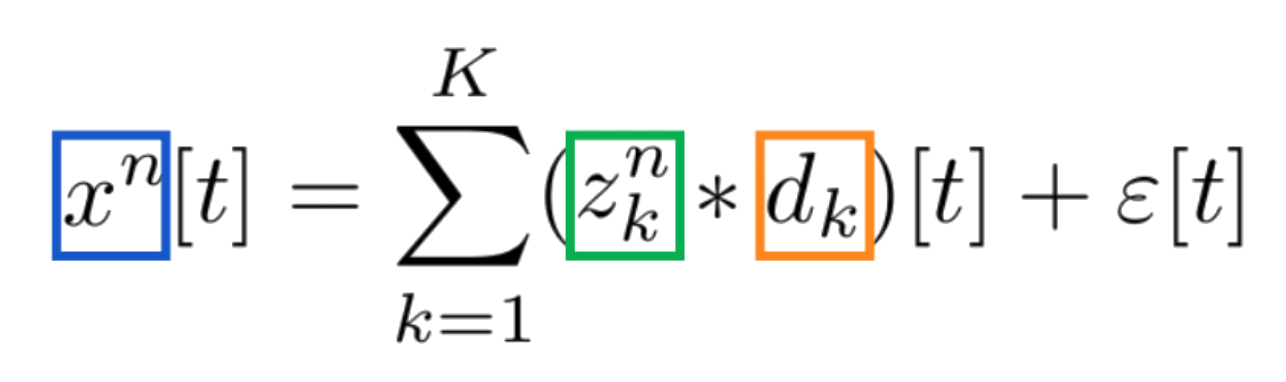
\includegraphics[width=.6\textwidth]{csc_explain_eq_color}%
    }
\end{frame}

\begin{frame}{Challenges de l'apprentissage non-supervisé pour les signaux}


%\begin{columns}[c]
%    \column{1em}
%    %\rotatebox{90}{\Large Formation}
%    \column{.9\textwidth}
%    \begin{block}{Computationnel}
%        \myitem Parallélisation \hskip3em \myitem Structure du dictionnaire\\[.5em]
%        \keypoint{[{\color{linkcolor} ICML, 2018; preprint, 2019}]}
%    \end{block}
%\end{columns}
%
%
%\begin{columns}[c]
%\column{1em}
%\rotatebox{90}{\Large Axe 1}
%\column{.9\textwidth}
%\begin{block}{Modélisation}
%    \myitem Activations \hskip1em \myitem Motifs\\[.5em]
%    \keypoint{[{\color{linkcolor} NeurIPS, 2018; ICASSP, 2019}]}
%\end{block}
%\end{columns}
%
%
%\begin{columns}[c]
%    \column{1em}
%    \rotatebox{90}{\Large Axe 1}
%    \column{.9\textwidth}
%    \begin{block}{Théorique}
%        \myitem Évaluation des atomes \hskip1em \myitem Garanties d'estimation\\
%        \myitem Optimization globale\\[.5em]
%        \keypoint{[{\color{linkcolor} NeurIPS, 2018; ICASSP, 2019}]}
%    \end{block}
%\end{columns}


\begin{itemize}\itemsep1.5em
    \item \textbf{Computationnel:} passage à l'échelle pour les longs signaux,
    \begin{itemize}\itemsep.5em
        \item[$\bullet$] Parallélisation.%
                         \keypoint{ICML 2018; preprint 2019}
        \item[$\bullet$] Utilisation de la structure du dictionnaire.%
                         \keypoint{ICLR 2017}
    \end{itemize}

    \item \textbf{Modélisation:} incorporer de la connaissance de domaine,
    \begin{itemize}\itemsep.5em
        \item[$\bullet$] sur les activations.%
                         \keypoint{ICASSP 2019}
        \item[$\bullet$] sur les motifs.%
                         \keypoint{NeurIPS 2018}
    \end{itemize}

    \item \textbf{Théorique:} qualité des motifs appris.
    \begin{itemize}\itemsep.5em
        \item[$\bullet$] Évaluation statistique des atomes.
        \item[$\bullet$] Garantie algorithmique de convergence globale.
        \item[$\bullet$] Garantie de reconstruction des motifs.
        \item[$\bullet$] Lien avec l'apprentissage profond.%
                         \keypoint{ICLR 2017}
    \end{itemize}
\end{itemize}


\end{frame}

\begin{frame}[t]{DICOD: Codage parcimonieux convolutif distribué%
              \keypoint{ICML, 2018}}
          
{\bf Obstacle computationnel:} Codage parcimonieux convolutif avec $\pmb D$ fixé:\vskip-.5em
\[
    \argmin_{Z_k} \| X - \sum_{k=1}^K Z_k * \pmb D_k\|_2^2 + \sum_{k=1}^K\|Z_k\|_1
\]
\only<1>{%
    \vskip1em
    {\large \bf Algorithmes existants:}\\[1em]
    \begin{itemize}\itemsep.5em
        \item Descente par Coordonnée Gloutonne\mycite{Kavukcuoglu2013}\\
            % {\small$\mathcal O(K^2T^2/q)$}
            \highlight{Itérations \small\color{black} $\mathcal O(KT)$}
            \highlight{Convergence \small\color{black} $\mathcal O(KT/q)$}
            \hskip1ex{\small$\Rightarrow\mathcal O(K^2T^2/q)$}
        \item Méthodes globales \mycite{Chalasani2013,Bristow2013}\\
             % {\small$\mathcal O(K^2TL/q)$}
             \highlight{Itérations \small\color{black} $\mathcal O(K^2TL)$}
             \highlight{Convergence \small\color{black} $\mathcal O(1/q)$}
             \hskip1ex{\small$\Rightarrow\mathcal O(K^2TL/q)$}
    \end{itemize}

    \vskip2em
    {\small\centering
    $T$:longueur du signal\hskip2ex
    $K$:nombre d'atomes\hskip2ex
    $L$:longueur des atomes\hskip2ex
    $q$:itérations\\}
}%
\vskip-1em
{
\centering
\inputTikZ{.7}{DICOD}\\[.5em]
}

\only<3->{
\begin{columns}[c]
    \column{.5ex}
    \techterm{Asynchrone}
    \column{.5ex}
    \techterm{Communications Locales}
    \column{.5ex}
    \techterm{Super-linéaire}
    \column{.5ex}
\end{columns}
\vskip-1em% {\bf Super linéaire:}
    \highlight{ Itérations \small\color{black} $\mathcal O(KT/W)$}
    \highlight{Convergence \small\color{black} $\mathcal O(KT/Wq)$}
    \hskip1em{\small$\Rightarrow\mathcal O(K^2T^2/\pmb {W^2}q)$}\\[.8em]
}%
%
\uncover<4>{%
    {\bf DiCoDiLe:} $\big[$
        \addstackgap[5pt]{\stackanchor[8pt]{Extension pour signaux 2D}
                                           {Complexité des itérations $\mathcal O(KL)$}} \keypoint{preprint 2019}\\
    \vskip.5em
    {\centering 
\includegraphics[height=.8em]{github}~\url{github.com/tommoral/dicodile}:
        Implémentation Python+MPI\\}
}

\end{frame}


\begin{frame}{Application aux Neurosciences \keypoint{NeurIPS, 2018}}

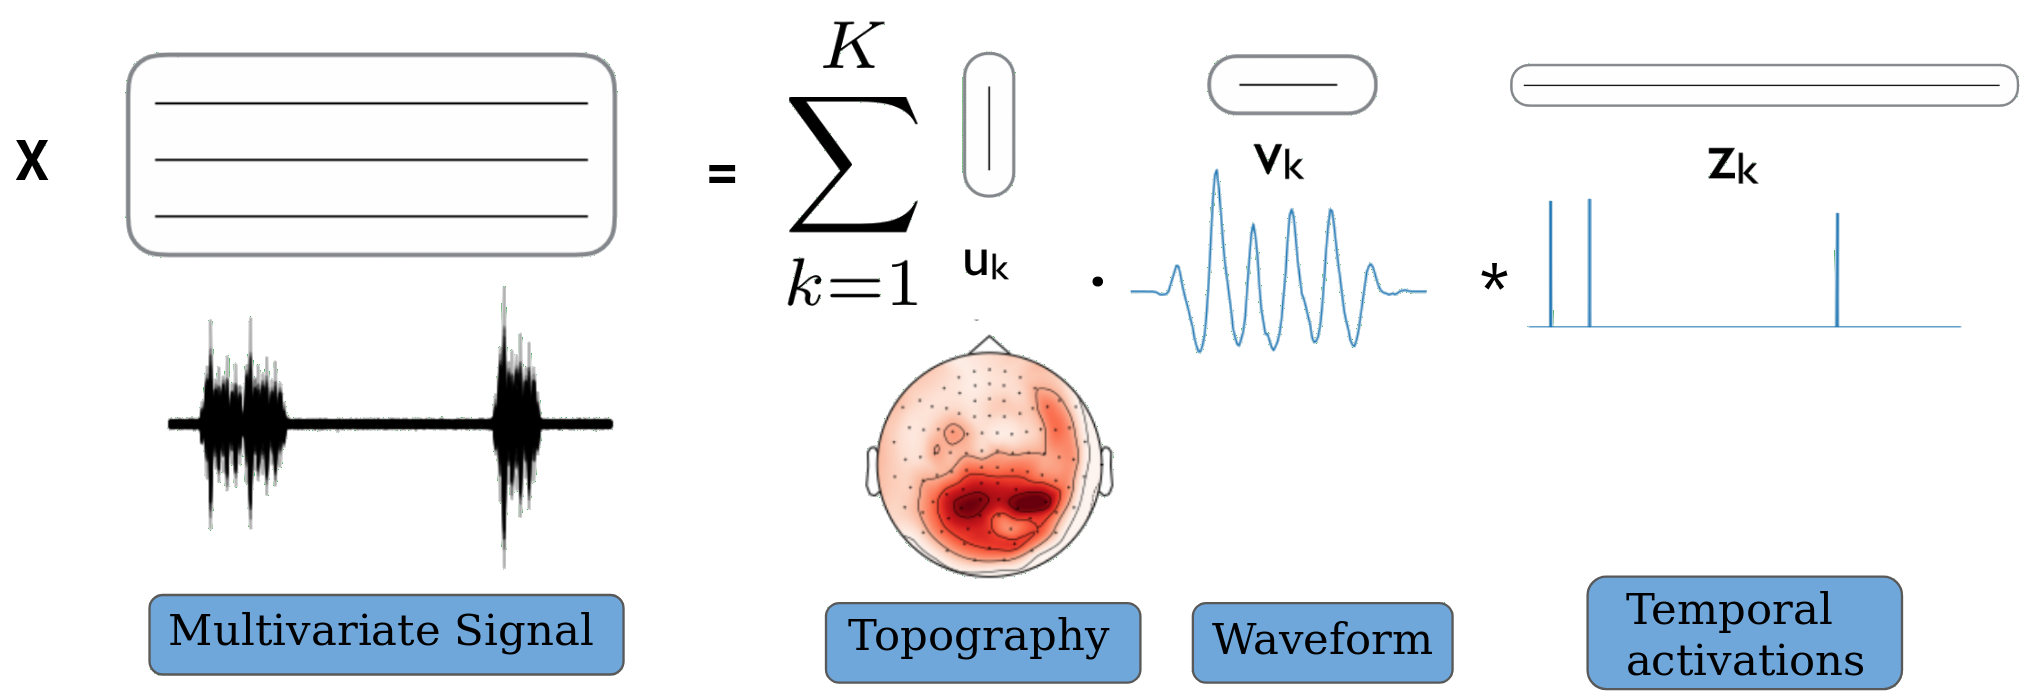
\includegraphics[width=\textwidth]{rank1}

\vskip1em
\begin{itemize}\itemsep.5em
    \item Modèle adapté à la physique des signaux MEG,
    \item Les atomes sont identifiables (réponses évoquées, artefacts, \dots)
    \item Les activations sont liées à la latence dans les signaux MEG de tâches.
\end{itemize}
\vskip3em
\centering

\includegraphics[height=.8em]{github}~\url{alphacsc.github.io}: librairie Python\\[1em]
\end{frame}

\begin{frame}{Projet de recherche}


\begin{columns}[c]
\column{1em}
\rotatebox{90}{\Large Axe 1}
\column{.9\textwidth}
\begin{block}{Modélisation pour les signaux en neurosciences}
    Identifier la structure dans le signal.\\[.3em]
    \myitem{} Dépendance temporelle \hskip2em \myitem{} Couplage fréquentiel\\[.3em]
\end{block}
\end{columns}
%
\vskip1em
\begin{columns}[c]
    \column{1em}
    \rotatebox{90}{\Large Axe 2}
    \column{.9\textwidth}
    \begin{block}{Analyse statistique des modèles convolutifs non-supervisés}
        Évaluer les modèles non-supervisé\\[.3em]
        \myitem{} Garantie de reconstruction \myitem Algorithme global.\\[.3em]
    \end{block}
\end{columns}
%
\vskip1em
\begin{columns}[c]
    \column{1em}
    \rotatebox{90}{\Large Axe 3}
    \column{.9\textwidth}
    \begin{block}{Apprentissage profond pour les problèmes inverses}
        Lien entre modèle convolutif et apprentissage profond.\\[.3em]
        \myitem Résolution rapide \myitem{} Identifiabilité de l'apprentissage profond.\\[.5em]
    \end{block}
\end{columns}

\end{frame}


\begin{frame}[t]{Modélisation pour les signaux en neurosciences \keypoint{Axe 1}}
\begin{columns}[T]
    \column{.5\textwidth}
    \centering
    \textbf{Comment mettre à jour les dépendances temporelles?}
    
    \vskip1em
    \centering
    \highlight{Modéliser les interactions}
    
    \alt<-3>{
        \raggedright\vskip1.5em
         Pénalité $\ell_1$\\[.3em]
            \hskip2ex$\Rightarrow$ activations indépendantes.\\[1em]
        \uncover<2->{Pénalités groupées (\eg{} $\ell_{1, 2}$)\\[.3em]
            \hskip2ex$\Rightarrow$ activations simultanées.\\[1em]}
        \uncover<3->{Processus ponctuels (\eg{} Hawkes)\\[.3em]
            \hskip2ex$\Rightarrow$ interactions temporelles.\\[1em]}
     }{
     \vskip.5em
     \highlight{Apprentissage auto-supervisé}\\

     \raggedright\vskip1.5em
     
     Prédiction de propriété \textit{ad hoc} \eg{}\\[.5em]
     
     \hskip1ex \raisebox{.1ex}{\small$\bullet$} à partir d'un segment, prédire T$_i$.\\[.5em]
     \uncover<5->{\hskip1ex \raisebox{.1ex}{\small$\bullet$} prédire $\Delta t$ entre 2 segments.\\[1em]}

     \uncover<6>{Dictionnaire adaptés à la tache\\[.3em]
                 \hskip1ex$\Rightarrow$ capture des effets temporels.}
    }
    
    \column{.5\textwidth}
    \centering%
    \only<1>{
        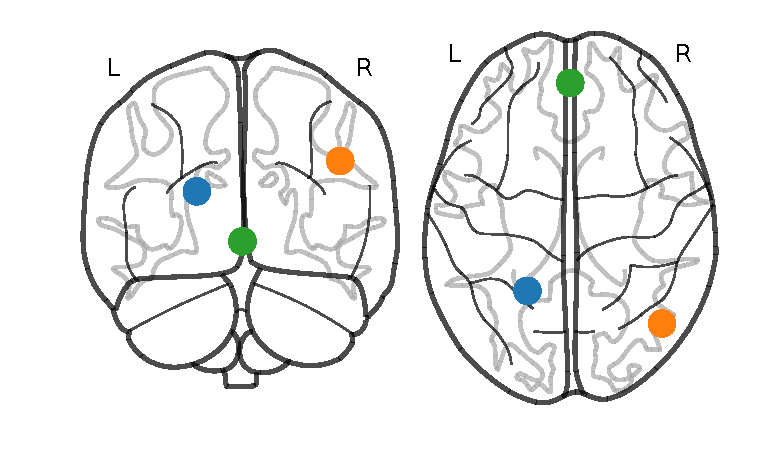
\includegraphics[height=8em]{connectivity_independent}
        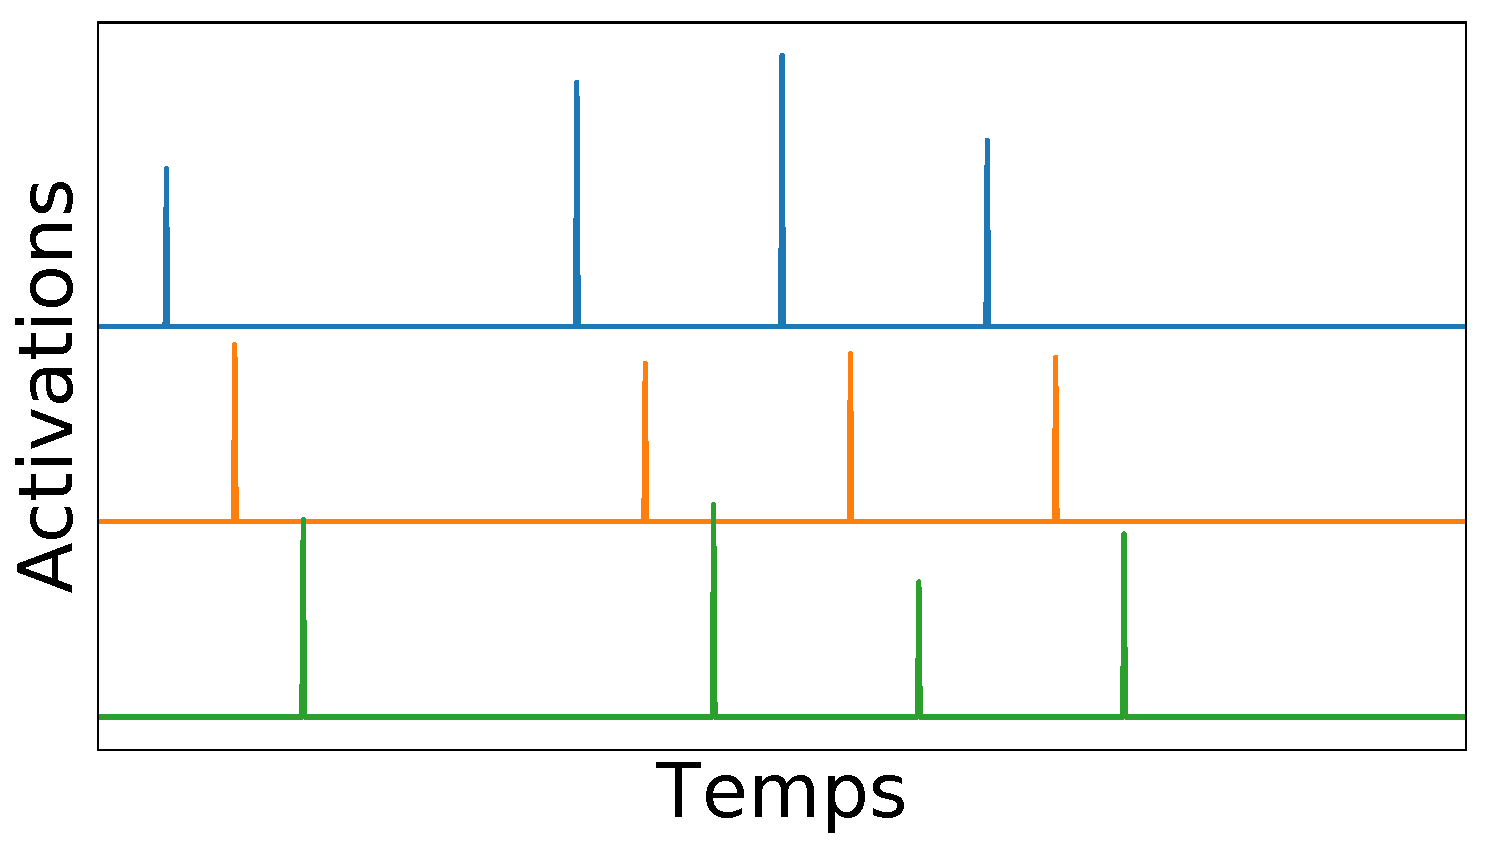
\includegraphics[width=\linewidth]{time_dependency}
        \centering\highlight[c=linkcolor]{Activations indépendantes}
    }%
    \only<2>{
        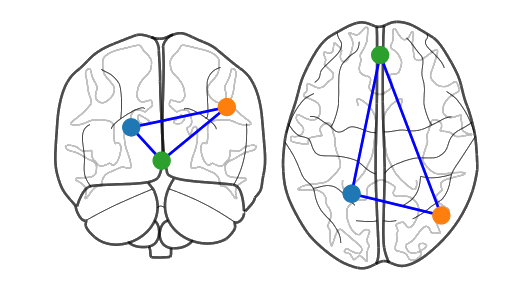
\includegraphics[height=8em]{connectivity_simultaneous}
        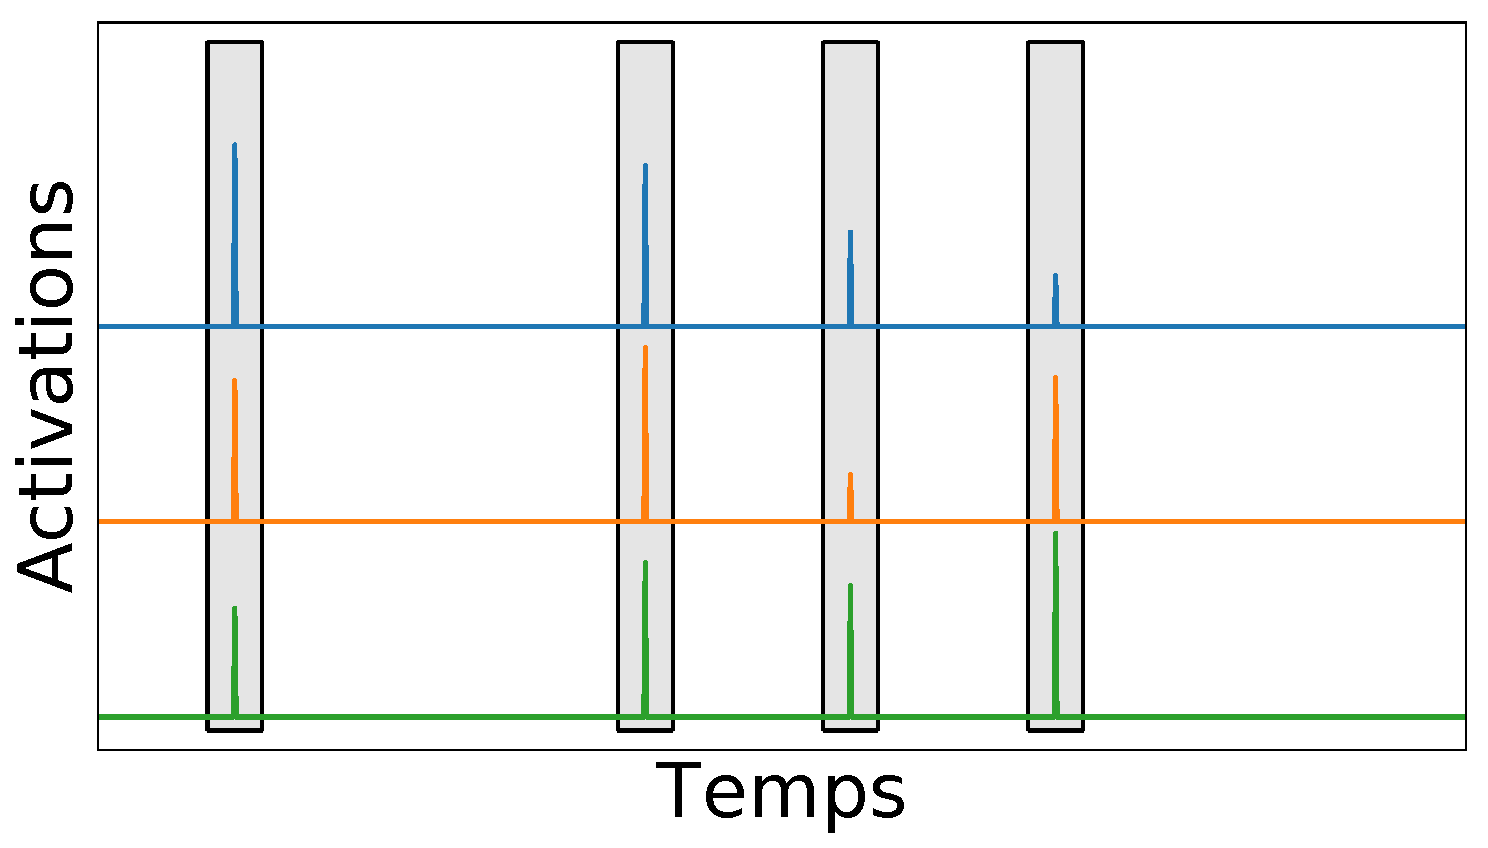
\includegraphics[width=\linewidth]{time_dependency_simultaneous}
        \centering\highlight[c=linkcolor]{Activations simultanées}
    }%
    \only<3>{
        \includegraphics[height=8em]{connectivity_default_mode}
        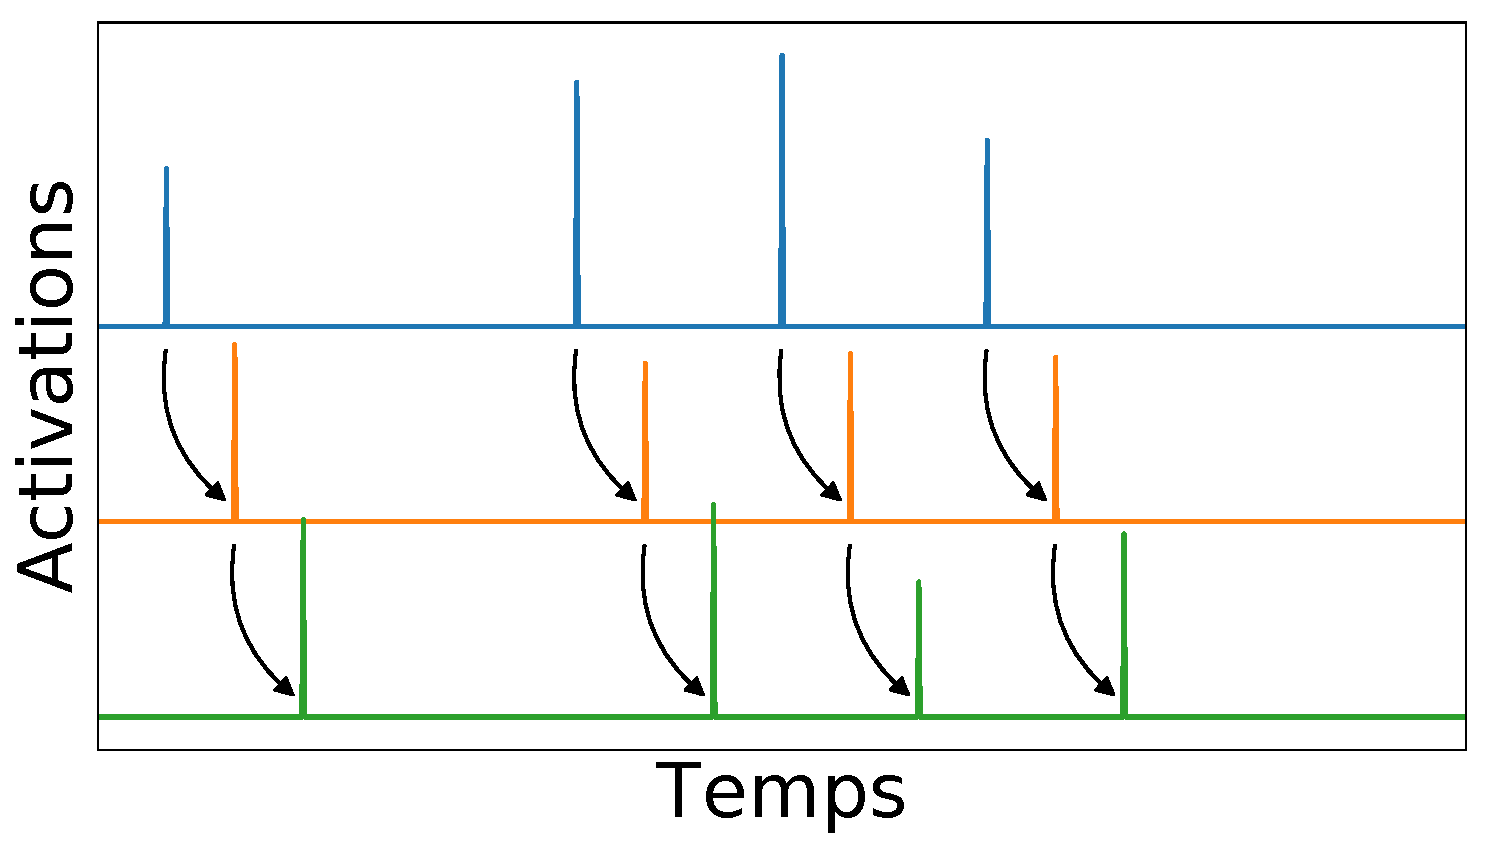
\includegraphics[width=\linewidth]{time_dependency_arrow}
        \centering\highlight[c=linkcolor]{Interaction temporelles}
    }%
    \only<4-6>{
        \vskip1em
        \alt<4>{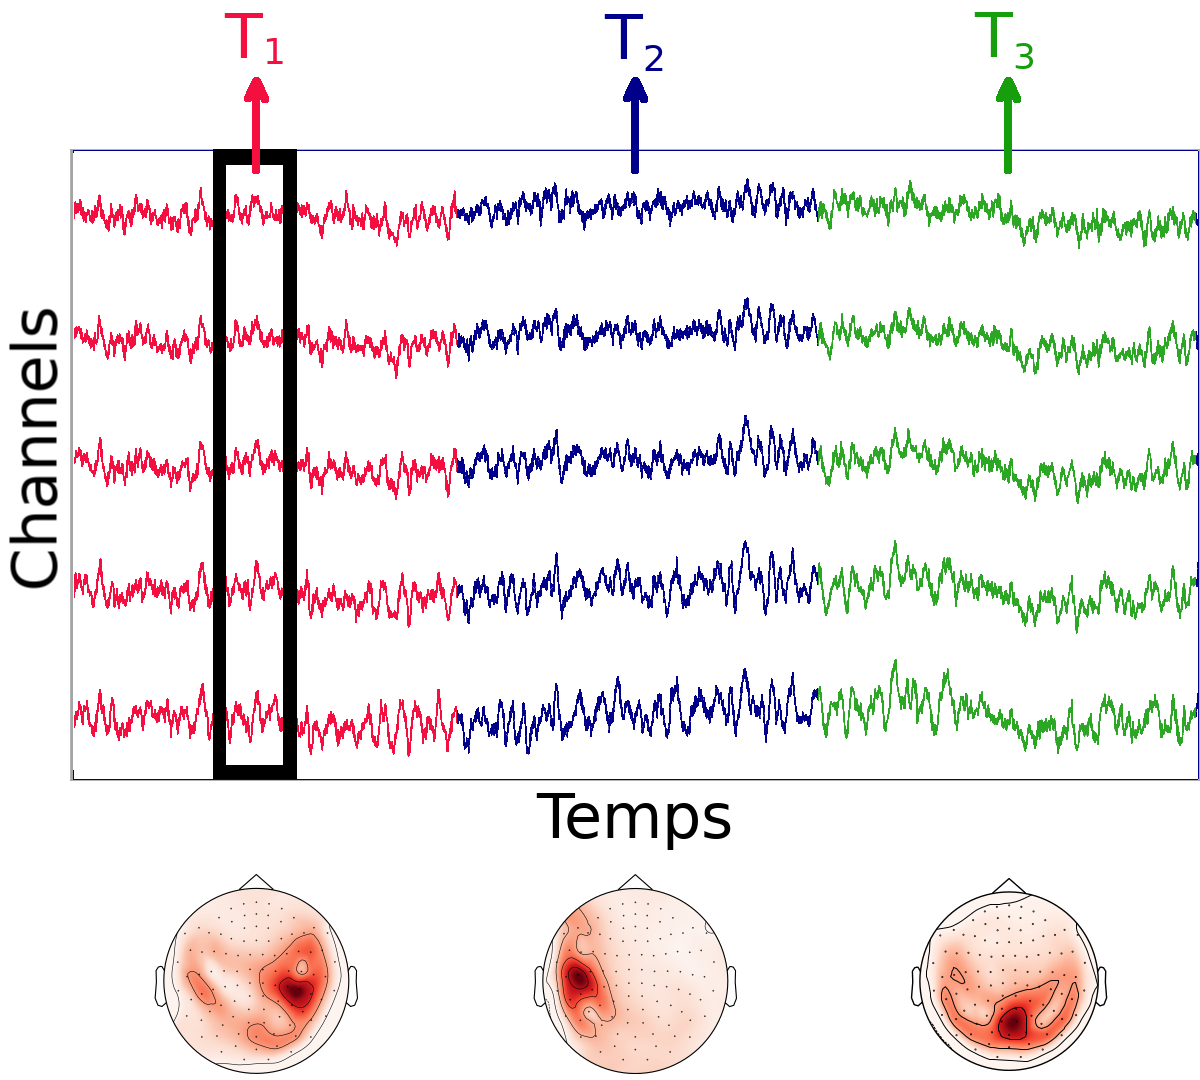
\includegraphics[width=\linewidth]{time_contrastive}
        }{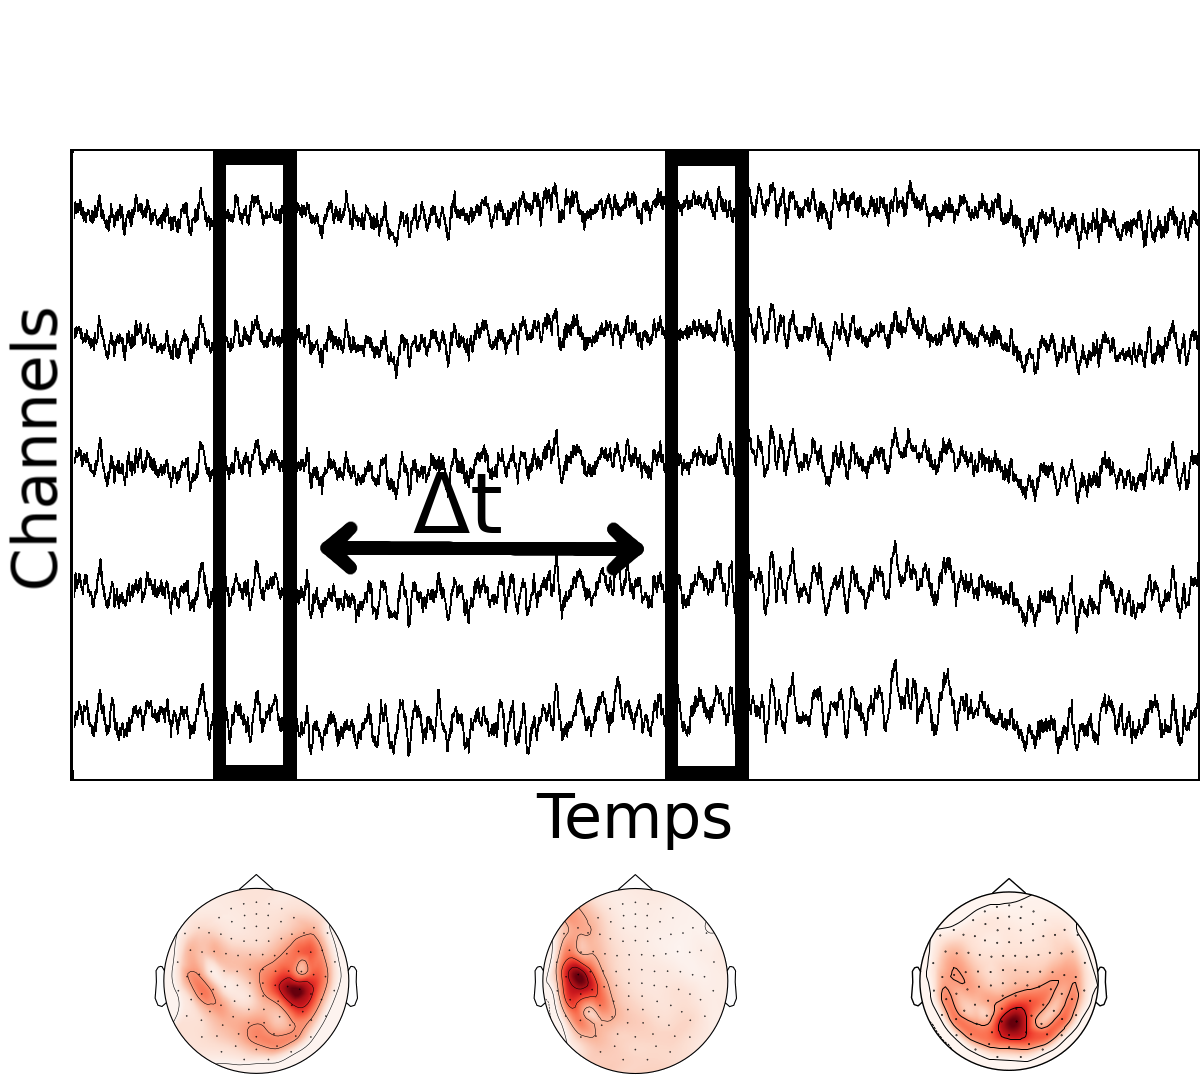
\includegraphics[width=\linewidth]{time_contrastive_delta_t}
        }
        \vskip1em
        \centering\highlight[c=linkcolor]{Non-stationnarité}
    }\\
\end{columns}

\end{frame}



\begin{frame}[t]{Analyse statistique des modèles non-supervisés \keypoint{Axe 2}}

{\centering \textbf{Comment évaluer les modèles non-supervisés?}\\[1em]}
\begin{tikzpicture}
    \coordinate (origin);
    \foreach \i in {0,...,2}{
        \node[inner sep=0em] (n\i) at (\i em, -\i em) {\includegraphics[width=4em]{meg_\i}};
    }

    \draw[densely dotted, <->, shorten >=1pt, shorten <=1pt] (n0.south west) -- (n2.south west);
         %node[midway, left] {N$_{\text{train}}$};

    \draw[->, black, thick, shorten >=3pt, shorten <=3pt] ($(n1.east) + (1em, 0)$) -- ++(5em, 0)
        node[midway, above] {\small Inférence}
        node[right] (atoms) {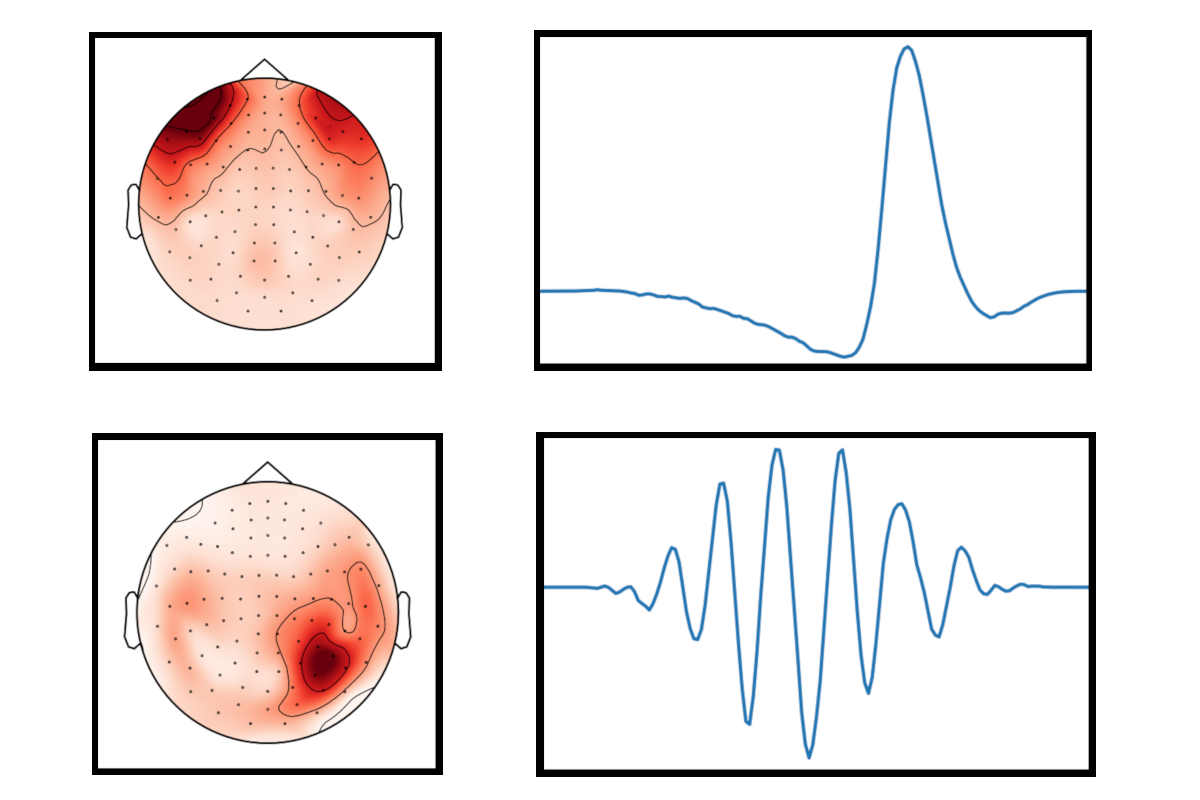
\includegraphics[width=5em]{meg_dict}};
    \draw[->, black, thick, shorten >=3pt, shorten <=3pt, dashed] (atoms.east) -- ++(6em, 0)
        node[midway, above] {\small Évaluation?}
        node[right, align=left, text width=5em] {Reconstruction?\\Débruitage?\\Génération?};
        
    % Labels
    \node[below=1em of n1, align=center] {\small Données\\\small d'entrainement};
    \node[below=0em of atoms] {\small Atomes};
\end{tikzpicture}
\vskip1em


\begin{columns}[c]
    
    \column{.5\textwidth}
    \uncover<2->{\centering
        \highlight{Stratégies d'évaluation}\\[1.5em]}
\begin{itemize}[<+(1)->]\itemsep1em
    \item Auto-évaluation
    \item Garanties de reconstruction
    \item Convergence globales
\end{itemize}

    \column{.5\textwidth}
    \only<2>{%
        \setlength{\bodywd}{\widthof{\bf Le modèle capture-t-il la}}
        \centering\highlight[c=linkcolor, wd=\bodywd]{%
                Le modèle capture-t-il la\\structure du signal?}\\[1em]
        Quantifier les structures identifiées par validation croisée.
    }%
    \only<3>{%
        \centering\highlight[c=linkcolor]{Le modèle est-il identifiable?}\\[1em]
        Utilisation de la structure fréquentielle des atomes.
    }%
    \only<4>{%
        \centering\highlight[c=linkcolor]{Le modèle peut-il être identifié?}\\[1em]
        Garantie de convergence basé sur les résultats récents pour la factorisation de matrice.
        
    }%
\end{columns}
\end{frame}
    
    
% \begin{frame}[t]{Analyse statistique des modèles non-supervisés \keypoint{Axe 2}}
%    \begin{columns}[T]
%        \column{2em}\vskip1em\rotatebox{90}{
%            \begin{beamercolorbox}[rounded=true, wd=13em, center]{title}
%                \large \bf Qualité des algorithmes
%            \end{beamercolorbox}
%        }
%        \column{.45\textwidth}
%        {\bf Garanties théoriques}\\[1em]
%        \begin{itemize}\itemsep.5em
%            \item Il est possible de designer un algorithme avec une preuve de convergence globale si $K$ n'est pas fixé
%            \item Analyse des propriétés de reconstruction théorique des motifs.
%        \end{itemize}
%        
%        
%        \column{2em}\vskip1em\rotatebox{90}{
%            \begin{beamercolorbox}[rounded=true, wd=13em, center]{title}
%                \large \bf Évaluation des modèles
%            \end{beamercolorbox}
%        }
%        \column{.45\textwidth}
%        {\bf Auto-évaluation}\\[1em]
%        \begin{itemize}\itemsep.5em
%            \item Apprendre un dictionnaire sur données d'entrainement.
%            \item Encoder la moitié des canaux des données tests.
%            \item Évaluer la reconstruction des autres canaux.
%        \end{itemize}
%    \end{columns}
%    \vspace{0pt plus 1 filll}
%    {\centering \textbf{Évaluation des modèles non-supervisés est un défi.}\\[1em]}
%\end{frame}


\begin{frame}[t]{Apprentissage profond pour les problèmes inverses \keypoint{Axe 3}}

\definecolor{Z}{RGB}{45,162,65}
\definecolor{F}{RGB}{180,35,35}
\begin{tikzpicture}
    \node (meg) {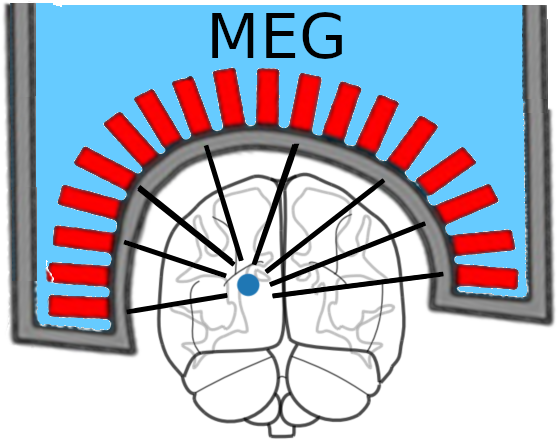
\includegraphics[width=9em]{meg_linear_propagation}};
    \draw[->, thick] ($(meg.east) - (0, 1.5em)$) -- ++(5em, 0)
        node[midway, align=center] (maxwell) {\small Équations\\ \small de Maxwell}
        node[right] (topomap) {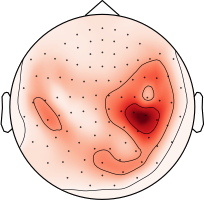
\includegraphics[width=4em]{topomap_somato}};
    \draw[->, thick] (topomap.east) -- ++(5em, 0)
        node[midway, align=center] {\small Problème\\ \small inverse}
        node[right] (brain) {\includegraphics[width=4em]{brain_activity}};
    \only<2->{
        \node[draw, rounded corners, above=2.5em] at (topomap.center) {
            \color{linkcolor} $\pmb X$};
        \node[draw, rounded corners, above=2.5em] at (brain.center) {
            \color{Z} $\pmb Z$};
        \node[draw, rounded corners, above=2.5em] at (maxwell.center) {
            \color{F} $\pmb F$};
    }
\end{tikzpicture}

\uncover<2->{
    \centering
    {\bf Problème inverse:} $\argmin_{\color{Z} \pmb Z} \|{\color{linkcolor} \pmb X}
                         - {\color{F} \pmb F}{\color{Z} \pmb Z}\|_2^2
                         + \mathcal R({\color{Z} \pmb Z})$\\[1em]
}


\begin{columns}[T]
    \column{.4\textwidth}
    \centering
    \uncover<3->{
        \highlight{\bf Optimisation apprise}\\[.5em]
    }
    \uncover<4->{
        \setlength\bodywd{\widthof{\bf Résolution rapide de}}
        \highlight[wd=\bodywd]{\bf Résolution rapide de problème inverse}\\[.5em]
    }
    \uncover<5>{
        \highlight[wd=\bodywd]{\bf Apprentissage profond identifiable}\\[.5em]
    }
    \column{.6\textwidth}
    \only<3>{
        \keypoint{ICLR 2017}\\[.5em]
        \centering
        \inputTikZ{.8}{ista_tikz}
        \setlength\bodywd{\widthof{\bf Dépend de la structure}}
        \highlight[c=linkcolor, wd=\bodywd]{Dépend de la structure de la Hessienne $F^\top F$}\\[1em]
    }
\end{columns}

\end{frame}


%===========================================================================
\section{Conclusion}
%===========================================================================


\begin{frame}{Intégration dans l’équipe/collaborations}

\begin{columns}[c]
%    \column{1em}
%    \rotatebox{90}{}
    \column{\linewidth}
    \begin{beamercolorbox}[rounded=true, shadow=true]{title}
        \vskip-.1em%
        {\color{black} \bf Parietal}\\[.3em]
        Modélisation neurophysiologique: \textcolor{linkcolor}{A. Gramfort; P. Ciuciu; D. Engemann}\\[.3em]
        Évaluation non-supervisée: \textcolor{linkcolor}{B. Thirion; G. Varoquaux}\\[.3em]
        Problèmes inverses rapides : \textcolor{linkcolor}{P. Ciuciu; A. Gramfort}\\[.3em]
    \end{beamercolorbox}
\end{columns}


\vskip.5em
\begin{columns}[c]
%\column{1em}
\column{\linewidth}
\begin{beamercolorbox}[rounded=true, shadow=true]{title}
    \vskip-.1em%
    {\color{black}\bf National}\\[.3em]
    Charactérisation des nystagmus chez le nourrisson:\\
        \hskip1em\textcolor{linkcolor}{M. Robert (CHU Necker); L. Oudre (UP13); 2 Étudiants (CMLA)}
\end{beamercolorbox}
\end{columns}


\vskip.5em
\begin{columns}[c]
%\column{1em}
\column{\linewidth}
\begin{beamercolorbox}[rounded=true, shadow=true]{title}
    \vskip-.1em%
    {\color{black} \bf International:}\\[.3em]
    Modélisation neurophysiologique: \textcolor{linkcolor}{B. Olshausen (Berkeley)}\\[.3em]
    Lien apprentissage profond et problème inverse: \textcolor{linkcolor}{J. Bruna (NYU)}.\\[.3em]
\end{beamercolorbox}
\end{columns}


\end{frame}


\begin{frame}[t]{Apprentissage non-supervisé pour les données de santé}%
\setlength{\parskip}{0em}
%
\begin{columns}[c]
    \column{2em}
    %\rotatebox{90}{\bf \large Parcours}%
    \column{.9\textwidth}%
    \begin{beamercolorbox}[rounded=true, shadow=true]{title}%
    {\large \bf \color{black} Parcours}\\
    2010-2014: X \hskip5.5em 2013-2014: Telecom ParisTech - MVA\\
    2014-2017: ENS Cachan \hskip.9em 2018-2019: Inria -- Parietal
\end{beamercolorbox}
\end{columns}%
%
\vskip1em
\begin{columns}[c]
    \column{2em}
    \rotatebox{90}{\parbox{4em}{\centering\large \bf Maths\\appli}}
    \column{.9\textwidth}%
    \begin{beamercolorbox}[rounded=true, shadow=true]{title}
\begin{columns}[c]
    \column{.85\textwidth}
        Méthodes non-supervisées \hskip2em Modélisation des signaux\\
        Lien apprentissage profond et optimisation\\
        Optimisation distribué\keypoint{4 actes de conférence}
    \column{.15\textwidth}
        \includegraphics[height=3em]{brain_and_signals}
\end{columns}
\end{beamercolorbox}
\end{columns}
\vskip1em
\begin{columns}[c]
    \column{2em}
    \rotatebox{90}{\parbox{4em}{\centering\bf \large Données\\Santé}}
    \column{.9\textwidth}%
    \begin{beamercolorbox}[rounded=true, shadow=true]{title}
    \begin{columns}[c]
        \column{.62\textwidth}
            Analyse de la marche \keypoint{2 articles; 1 brevet}\\
            Mouvements oculaires \keypoint{3 articles soumis}\\
            Neurosciences \keypoint{2 actes de conférence}\\
        \column{.38\textwidth}
            \centering
            \includegraphics[height=3em]{logo_cognac}
            \includegraphics[height=3em]{logo_neurospin}
    \end{columns}
    \end{beamercolorbox}
\end{columns}
\vskip.7em
\begin{columns}[c]
    \column{2em}
    \rotatebox{90}{\parbox{4em}{\centering\bf \large Logiciel\\Libre}}
    \column{.9\textwidth}%
    \begin{beamercolorbox}[rounded=true, shadow=true]{title}
        \begin{columns}[c]
            \column{.5\textwidth}
             Calcul parallèle en Python\\
            Développeur pour 3 librairies\\
            Contributeur pour 2 projets
            \column{.5\textwidth}
            \centering
            \includegraphics[height=3em]{logo_python}
            \includegraphics[height=3em]{logo_joblib}
            \includegraphics[height=3em]{logo_sklearn}
        \end{columns}
    \end{beamercolorbox}
\end{columns}

\end{frame}


%\begin{frame}{Profile}
%\begin{columns}[T]
%    \column{.33\textwidth}
%    \textbf{Machine Learning}\\
%    
%    \begin{itemize}
%        \item Unsupervised pattern recognition, Optimization
%        \item 3 papers in major conferences
%        \item 
%    \end{itemize}
%    \column{.33\textwidth}
%    \textbf{Open-source Software}
%    \begin{itemize}
%        \item Parallel computing in python
%        \item Core-developer of joblib (parallel computation engine for scikit-learn)
%        \item Contributed to important OSS projects (python, scikit-learn, ...)
%    \end{itemize}
%    \column{.33\textwidth}
%    \textbf{Applications}
%    \begin{itemize}
%        \item Oculographic recordings
%        \item Equilibrium assessments
%        \item Neuroscience
%    \end{itemize}
%\end{columns}
%\end{frame}
%===========================================================================
% AUXILIARY SLIDES
%===========================================================================



%===========================================================================
\appendix
\section{Auxiliary Slides}
%===========================================================================


%===========================================================================
\subsection{Aux1}
%===========================================================================
%
%\begin{frame}{Auxillary slide 1}
%
%\end{frame}
%
%
%\begin{frame}{}
%\vskip2em
%{\centering
%    \usebeamercolor[fg]{title}
%    \usebeamerfont{title}
%    \Huge \bf Merci!\\[2em]}
%
%Code available online:\\[1em]
%
%%
\includegraphics[height=.8em]{github}~\textbf{LISTA} : github.com/tommoral/AdaptiveOptim\\[1em]
%
%
\includegraphics[height=.8em]{github}~\textbf{alphacsc} :  \url{alphacsc.github.io}\\[2em]
%
%Slides are on my web page:\\[1em]
%\hskip5em\includegraphics[height=.8em]{website} \url{tommoral.github.io}
%\hskip4em 
\includegraphics[height=.8em]{twitter} \href{https://twitter.com/tomamoral}{@tomamoral}
%
%
%\end{frame}
%

\end{document}
